\documentclass[paper=a4, fontsize=11pt]{scrartcl} 

\usepackage[T1]{fontenc} 
\usepackage[english]{babel}
\usepackage{amsmath,amsfonts,amsthm}

\usepackage{lipsum}

\usepackage{graphicx}
\usepackage{float}
  \floatplacement{figure}{H}
  \floatplacement{table}{H}
  
\usepackage{sectsty} 
\allsectionsfont{\centering \normalfont\scshape} 

\usepackage{fancyhdr} % Custom headers and footers
\pagestyle{fancyplain} % Makes all pages in the document conform to the custom headers and footers
\fancyhead{} % No page header - if you want one, create it in the same way as the footers below
\fancyfoot[L]{} % Empty left footer
\fancyfoot[C]{} % Empty center footer
\fancyfoot[R]{\thepage} % Page numbering for right footer
\renewcommand{\headrulewidth}{0pt} % Remove header underlines
\renewcommand{\footrulewidth}{0pt} % Remove footer underlines
\setlength{\headheight}{13.6pt} % Customize the height of the header

\numberwithin{equation}{section} % Number equations within sections (i.e. 1.1, 1.2, 2.1, 2.2 instead of 1, 2, 3, 4)
\numberwithin{figure}{section} % Number figures within sections (i.e. 1.1, 1.2, 2.1, 2.2 instead of 1, 2, 3, 4)
\numberwithin{table}{section} % Number tables within sections (i.e. 1.1, 1.2, 2.1, 2.2 instead of 1, 2, 3, 4)

\setlength\parindent{0pt} % Removes all indentation from paragraphs - comment this line for an assignment with lots of text

%----------------------------------------------------------------------------------------
%	TITLE SECTION
%----------------------------------------------------------------------------------------

\newcommand{\horrule}[1]{\rule{\linewidth}{#1}} % Create horizontal rule command with 1 argument of height

\title{	
\normalfont \normalsize 
\textsc{Computational Science - ITB} \\ [25pt] % Your university, school and/or department name(s)
\horrule{0.5pt} \\[0.4cm] % Thin top horizontal rule
%\huge  Summary - Euler Method\\ % The assignment title
%\horrule{2pt} \\[0.5cm] % Thick bottom horizontal rule
}

\author{\small{Ridlo W. Wibowo || 20912009}} % Your name

\date{\normalsize\today} % Today's date or a custom date

\begin{document}

\maketitle % Print the title

\section{Summary - Euler Method}
Euler method is first order single-point method for solving ordinary differential equations (ODEs) with a given initial value (IV). It is the most bacic explicit method for numerical integration of ODEs and the simplest Runge-Kutta method. Although this method is too inaccurate to be of much practical value, it's useful to illustrate many concepts relevant to the finite difference solution of initial-value ODEs.
\\
Consider the general nonlinear first-order ODE:\\
\begin{equation}
\overline{y}' = f(t, \overline{y})  \hspace{2.0cm} \overline{y}(t_{0}) = \overline{y}_{0}
\end{equation}

From Taylor series:
\begin{equation}
\overline{y}_{n+1} = \overline{y}_{n} + \Delta t \overline{f}_{n} + \dfrac{1}{2} \overline{y}'' (\tau_{n}) \Delta t^{2} = \overline{y}_{n} + \Delta t \overline{f}_{n} + O(\Delta t^{2})
\end{equation} 

Truncating the remainder term, which is $ O(\Delta t^{2}) $, and solving for $ y_{n+1} $ yields the \textit{explicit Euler} finite difference equation (FDE):
\begin{equation}
y_{n+1} = y_{n} + \Delta t f_{n}  \hspace{2cm} O(\Delta t^{2})
\end{equation}
where the $ O(\Delta t^{2}) $ term is included as a reminder of the order of the local truncation error.\\
Several features of above equation are summarized below:
\begin{enumerate}
\item The FDE is explicit, since $f_{n}$ does not depend on $y_{n+1}$.
\item The FDE requires only known point. Hence, it is a single point method.
\item The FDE requires only one derivative function evaluation [i.e. $f(t,y)$] per step.
\item The error in calculating $y_{n+1}$ for a single step, the local truncation error, is $O(\Delta t^{2})$.
\item The global (i.e. total) error accumulated after $N$ steps is $O(\Delta t)$.
\end{enumerate}

At the final point $t_{N}$: 
\begin{equation}
y_{N} = y_{0} + \sum (y_{n+1} - y{n}) = y_{0} + \sum \Delta y_{n+1}
\end{equation}

and the total truncation error is given by,
\begin{equation}
\label{err}
Error = \sum \frac{1}{2} y'' (\tau_{n}) \Delta t^{2} = N \frac{1}{2} y'' (\tau) \Delta t^{2},
\end{equation}

where $t_{0} \leq \tau \leq t_{N}$, so the number of steps $N$ is related to the step size $\Delta t$ as follows:
\begin{equation}
\label{jum}
N = \frac{t_{N} - t_{0}}{\Delta t}
\end{equation}

Substituting \eqref{jum} to \eqref{err} yields:
\begin{equation}
Error = \frac{1}{2} (t_{N} - t_{0}) y'' (\tau) \Delta t = O \Delta t
\end{equation} 
Consequently, the global (i.e. total) error of the \textit{explicit Euler} FDE is $O \Delta t$.
\\
\\
The other first-order single-point method for FDEs is \textit{implicit Euler} method. There are many second-order method from Euler method  which is generally called the modified Euler method. Runge-Kutta is fourth-order single-point method, and there are many higher order by modifying this method.  

\begin{figure}
	\centering
	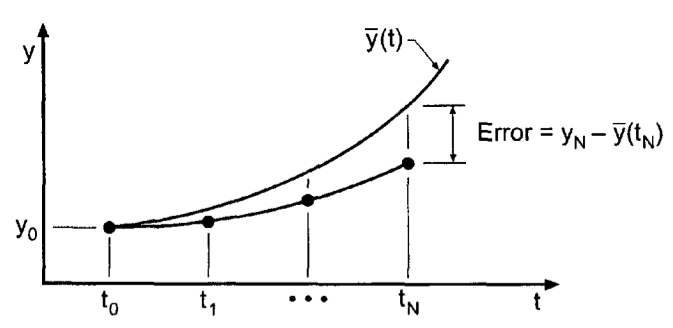
\includegraphics[width=0.8\textwidth]
		{eulerexplicit.png}
	\caption{Repetitive application of the explicit Euler method.}
	\label{fig:keplerian}
\end{figure}


\end{document}
